\chapter{Financialization} \label{chapter-financialization}
\epigraph{Financialization  occurs when housing is treated as a commodity—a vehicle for wealth and investment—rather than a social good.}{Special UN Rapporteur on the right to adequate housing, Leilani Farha}
%https://www.ohchr.org/en/special-procedures/sr-housing/financialization-housing
\epigraph{Financialization is a process whereby financial markets, financial institutions, and financial elites gain greater influence over economic policy and economic outcomes. Financialization transforms the functioning of economic systems at both the macro and micro levels.}{Thomas I. Palley \cite{palleyFinancializationWhatIt2007}}
%*** ADD MORE ON THE LITERATURE ON FINANCIALIZATION TO SETUP OUR WORK, AS IN THE ABOVE CHAPTERS
In this thesis we are focused on modelling the  effects of financialization on the urban housing market.  The term financialization is used in a variety of way across a fairly wide range of contexts. In finance, it is  a term for the process of developing the legal instruments that facilitate financial transaction.  At the microeconomic level it is  a  collective noun for the huge number of individual transactions, that create or transfer a financial assets. At a macro level it refers to the effect on the system itself of the new instruments and the increase in the type of transaction that they make possible.

We therefore begin in Section~\ref{section-financialize}  with a narrow definition of the act of financializing, followed by  an explanation and examples. In Section~\ref{section-micro} we describe the microeconomic objective function that individuals and our bank agent  employ in deciding to purchase a property. Finally, in  
In Section~\ref{section-system} we explain how the term is applied at the level of systems and while markets. At that point we can introduce our specific hypotheses and how we intend to test them.
% We therefore begin with a narrow and strict definition of the act of finacializing, followed by  an explanation and examples. We then go on to explain how the term is applied at the level of systems and while markets.

% At that point we can introduce our specific hypotheses and how we intend to test them.

\section{Financial instruments and financialization} \label{section-financialize}
The word ``financialization'' has several quite different meanings.  

%*YOU SAY ABOVE YOU ARE GOING TO NARROW TO A SPECIFC DEFINITION, CAN YOU MAKE VERY CLEAR HERE WHAT THAT IS. LIKE THESE ARE ALL POSSIBLE DEFINITIONS. THEN STATE VERY EXPLICITLY, THIS IS THE ONE WE ARE USING. 

To financialize anything is to create a  \gls{financial instrument} that represents it and can be bought and sold as an investment. Not all financial instruments are instruments of financialization. For example, mortgages are  financial instruments, but another step is required to create a financialized  market in mortgages. 
*E i'M A BIT CONFUSED HERE... i THINK YOU ARE GOING INTO EXPLAINING HOW THEY BECAME FINANCIALIZED, BUT IT'S SET UP LIKE AND EXAMPLE... CAN YOU SAY WHERE YOU ARE GOING BEFORE OPENING THE DETAILS ABOUT THE MORTGAGE. lIKE THEY BECAME FINACICLAIZED OVER TIME... AT A BASI LEVEL A MORTGAGE MAKES POSSIBLE ETC..

A mortgage  makes possible a specific transaction between one potential seller and a potential buyer. The buyer and the seller both want to transfer the ownership in exchange for a sum of money, but the buyer may not have the amount required in the present. The mortgage instrument makes the transaction possible by createing a legally binding commitment to satisfactory future payment by conferring on the initial owner the right to repossess his property if the terms of the agreement are not met. The security provided by this instrument ``de-risks'' the transaction, making it safer and therefore easier to achieve the mutual benefits of the sale. %Buyers would get loans directly from the seller – no banks or outside parties were involved. 

Originally mortgages were an arrangement between just the buyer and the seller, but in the 1870s in the USA, insurance companies stepped into these transactions, paying off the seller and then collecting the principle and interest payments on behalf of the bank's shareholders. This innovation was an example of financialization that made it possible for individual insurance companies to profit by providing money to buyers.   When mortgage lending was regulated and insured  by the American government during and after the great depression it facilitated a massive increase in home ownership in the USA and contributed to the post-war construction boom and the suburbanization of American cities. 


These mortgages were still agreements between individual lenders and buyers. When financial institutions developed markets that let them buy and sell bundles of mortgages among themselves, we say the mortgage market itself was financialized. There was then a market for the  promises to pay in addition to the underlying market for housing and the market for mortgage-type loans loans

The transactions in this market do not directly affect the mortgage conditions or the home: they simply added a new product for investors or banks  to buy and sell. This new market was thought to further reduce the risk for lenders, but  between 2007 and 2010 in the USA the sub-prime mortgage crisis destabilized the financial institutions that were playing this new market. \footnote{As I understand it, that crisis resulted from overselling risky and predatory mortgages by lenders with more money to lend than the market could absorb. Eager investors seeking higher or more secure returns were willing  to buy supposedly de-risked bundles of  mortgages. (The instruments that enabled the speculative bubble were mortgage-backed securities (MBSes) and collateralized debt obligations (CDOs).) As it turned out, mortgage defaults rose, lenders' liquidity fell, rates rose, defaults increased and the market for the new instruments collapsed, taking down major financial institutions. The details don't matter for this thesis. }.  
*E IF YOU SAY IT WAS THOUGHT TO LOWER RISK, CAN YOU FINISH THAT THOUGHT. %DID THE CRISIS SHOW IT DIDN'T? OR IS IT UNCLEAR WHETHER IT DOES? iS IT A DEBATED POINT? OR CHEANGE THE SENTENCE SO YOU DON'T SET UP IT WAS THOUGHT AND LEAVE THE CONCLUSION HANGING...

Recently, the creation of \glspl{REIT}, Real Estate Investment Trusts, allowed investors to buy shares in a fund that buys properties, giving them a share of the revenue and any speculative gains the fund achieves.



\section{The rate of return on a property purchase}\label{section-micro}

At  the microeconomic level, where individual decisions are made, financialization is the purchase of assets  like homes for the sake of the  future stream of revenue and speculative gains it offers. Real assets are bought by individuals and institutions looking to maximize the return on the financial resources they have, and thereby become financial assets. The real asset takes on an additional and separate economic meaning as financial object that can be bought and sole.

investment of this sort is mediated by financial institutions on behalf of the owners of the financial assets, 

Financialization at this level is a term for the a process  mediated by financial institutions on behalf of the owners of the financial assets that increase the stock of financial assets associated with a stock of real assets. %it may be understood as the process by which which financial institutions,  increase in size and influence. 
% ADD TABLE WITH VARIABLE DEFINITIONS
 
% The rule has long run implications for the ownership of housing. 
% *THIS SECTION SEEMS LIKE A JUMP... HAT IS THE CONTEXT? WHAT RULE?

%The implications of {\color{red} Equation~\ref{eqn-property-investment-return1}} are significant for the evolution of the urban land market and class structure.  
Some of the implications include:

\begin{enumerate}
\item A large $m$ magnifies the return. (The downpayment is smaller as a fraction of the price, increasing the investor's leverage). 

\item A lower mortgage interest rate increases the return by lowering interest payments.  The wealthy can generally borrow  at lower interest rates than the less wealthy. 

\item A lower discount rate $\delta$ reduces the subjective rate of return.  \footnote{Poverty in assets, or cash liquidity constraints, was leading to or correlated with higher rates of time preference \cite{HoldenShiferaw--1998}. Poverty, market imperfections and time preferences: of relevance for environmental policy?   S. Holden, B. Shiferaw, M. Wik.  1998, Environment and Development Economics https://www.semanticscholar.org/paper/Poverty %2C-market-imperfections-and-time-preferences%3A-Holden-Shiferaw/55376ceb29b6f3bab2d8fb3dd83d5904826959ac
}
\item Higher expected price appreciation increases the attractiveness of investment. The wealthy and financial corporations  are likely to have better price forecasts than  the occasional home buyer.
\item Higher rents make the unit more profitable. higher expected  rents may result from expecting greater price appreciation raises expected profitability or greater willingness to raise rents for tenants 

\item Lower maintenance costs increase profits. There may be scale economies in the maintenance  of rented housing. 
\item Lower tax rates decrease holding costs and increase the value of the investment. here may be opportunities to shelter income with land held for investment (speculative) purposes
\end{enumerate}
%As expected
%\begin{enumerate}
%\item A large $m$ magnifies the return. (downpayment is smaller)
%\item A lower mortgage interest rate increases the return because of interest on the mortgage
%\item A lower discount rate $\delta$ reduces the subjective rate of return
%\item Higher expected price appreciation increases the attractiveness of investment
%\item Higher rents makes the unit more profitable if rents are being collected
%\item Lower costs increase profits
%\item Lower tax rates decrease holding costs and increase the value of the investment
%\end{enumerate}

Since interest rates are lower for those with higher wealth, the analysis implies, consistent with the empirical evidence, that net returns for investment are increasing with wealth. Large wealth holders will get higher expected and actual rates of return on land than those with lower wealth holdings. Managers of large pools of capital will have an even greater advantage. \footnote{ Equation~\ref{Eqn:DecisionRule} implies a `bang-bang' *** DEFINE control - with all sales going to the richest participant unless there are limits on the size of capital flows. For our simulation, we implement such limits. } \footnote{Furthermore, given the  common rule that mortgage payments cannot exceed some fraction of disposable income, the wealthy will be able to borrow larger amounts and at lower interest rates than the less wealthy. At any distance from the centre they will be able to make a higher bid.} %The cost of capital is known to differ for rich and poor. The implication is that those with more capital will be at an advantage in the urban housing  market. 
Tax treatment of income and capital gains as well as interest deductibility will also influence Equation~\ref{Eqn:DecisionRule}'s strength and who benefits most. \footnote{Case and Schiller \cite{CaseandSchiller} observe that (source?) 
`` ... increases in real per capita income all are positively related to excess returns or price changes over the subsequent year.''} 
\footnote{Fr\'ed\'erick Demers found that the response of housing investment to interest rates has become more pronounced over time \cite{FredrickDemers}. Modelling and Forecasting Housing Investment: The Case of Canada,  Research Department, Bank of Canada, Ottawa, Ontario, Canada K1A 0G9 fdemers@bankofcanada.ca *** ELABORATE} 

Some  of these conditions (1-3) hold generally for wealthier actors. Others (4-7) may be available only to institutional investors.  Financial corporations in particular may have advantages relative to individual investors, making it  reasonable to expect that financial corporations increasingly dominate urban land markets. %A recent report claimed 15\% of Tioron0's land transa

\begin{enumerate}
\item Given the  common rule that mortgage payments cannot exceed some fraction of disposable income, the wealthy will be able to borrow larger amounts and at lower interest rates than the less wealthy. At any distance from the centre they will be able to make a higher bid.

\item The cost of capital is known to differ for rich and poor. \footnote{Fr\'ed\'erick Demers \cite{FredrickDemers} found that the response of housing investment to interest rates has become more pronounced over time. Modelling and Forecasting Housing Investment: The Case of Canada,  Research Department, Bank of Canada, Ottawa, Ontario, Canada K1A 0G9 fdemers@bankofcanada.ca} 


\item If agents discount at their borrowing rate, wealthier agents may have a lower subjective rate of time preference and therefore value properties more highly. 
\end{enumerate}
The implication is that those with more capital will be at an advantage in the urban housing  market. Tax treatment of income and capital gains as well as interest deductibility will influence Equation~\ref{Eqn:DecisionRule}'s strength and who benefits most. 

\begin{itemize}
\item The effect of increasing the urban workforce is to increase the marginal products of  both capital and labour throughout the urban economy.% This premium on production in cities is positive when $\Lambda'$ is greater than zero.
 \item  As long as $\Lambda'>0$ cities will  grow, potentially leading to the ``catastrophic agglomeration''  that has been noted in other models.  (\cite{fujitaSpatialEconomyCities1999, baldwinAgglomerationRegionalGrowth2004, krugmanIncreasingReturnsEconomic1991, gurwitzCatastrophicAgglomeration2019}).%  City size could be bounded, in which case the city system would grow by increasing the number of cities. This appears to depend on the model features and parameters. 
%\item Cities will draw investment away from rural and remote areas.
%\item Cities will draw labour away from rural and remote areas. 
\item Even in competitive markets, capital captures scale benefits until an entry equilibrium is achieved.
\item Landowners  capture the agglomeration benefits that are not dissipated in transportation costs.
\end{itemize}

These appear to be features of the economy we observe.


\section{Financialization as system change}\label{section-system}


Financialization of the housing market is therefore the increasing control of the stock of urban land and housing in order to capture the scarcity rent generated by the people of the city.  Mortgages and REITs are both financial instruments.
*e tHIS IS CLEAR BUT COULD BE HELPED BY RESTATING HOW THEY MOVE IT ONTO FINANCIAL MARKETS. JUST A QUICK SUMMARY STATEMENT OF HOW THEY ARE FINACIALIZATION. %EVEN JUST something like... They put the ownership of housing onto financial markets. just to keep us oriented in what we are talkign about.

*E I FEEL LIKE THERE IS SOMETHING MISSING BETWEEN THESE TWO PARGRAPHS. %PERHAPS JUST FLESHING OUT WHAT FINANCIALIZATION LOOKS LIKE TECHNICALLY. MAYBE ALSO INSTRODUCE POSIBLE EFFECTS... LIKE EVEN JUST INTRODUCE THEM AS QUESTIONS? IT'S BEEN SUGGESTED OR SHOWN THAT ITS CONTRIBUTING TO THE HOUSING CRISIS. tHIS WOULD ALSO BE A GOOD PLACE TO EXAPLIN WHAT YOU MEAN BY "aS SYSTEMS CHANGE... BECAUSE i THINK THAT IS A BIG PART OF WHY YOU SAY NEXT THAT IT NEEDS TO BE UNDERSTOOD... BECAUSE IT HAS SUC BROAD EFFECTS

We need to understand the economics of financialization.
% \section{Literature on theory and evidence} % PROVIDE EVIDENCE 	mention theories?
There is substantial evidence that the financialization of urban housing is underway in Canadian cities..

Two questions arise when we observe the growing participation of global capital in the urban housing system: 
\begin{enumerate}
\item How far will the financialization of urban land go? 
\item That are the implications for the urban economy and the welfare of the urban population? 
\end{enumerate}

We can demonstrate that in the absence of policy interventions, differential access to finance capital ensures that capital owners acquire an increasing share of urban land % over time
and therefore capture the growing land rents from urban productivity growth. 

With this insight, growing wealth inequality emerges within a simple, widely accepted model of the urban land market. In the limit, urban residents are tenants, and new residents without capital no longer receive any of the increases in rents arising from the growing productivity of the city. 

%The first question, therefore, is reduced to which capital holders will increase their share of urban land and whether there is any reason to expect the process of financialization process to stop or reverse itself.

% \section{The incentives for financialization}
%Instead, drawing on the ideas of Jane Jacobs, Lucas proposes the city as the unit of analysis. Lucas, Robert (1990), "Why Doesn't Capital Flow from Rich to Poor Countries?," American Economic Review Papers and Proceedings v. 80, no. 2 (May) pp. 92-96.  
%Jacobs, Jane  (1969), The Economy of Cities (New York: Random House).  
% The Death and Life of Great American Cities \cite{jacobsDeathLifeGreat1961}


 MOVE The mortgage share and interest rate are functions of the agents wealth %Both the  share of the price  that can be mortgaged, $m$, and the interest rate and the interest rate paid, $r$, are functions of the agent's wealth. 
The discounting factor may be correlated with wealth as well. 

%%%%%%%%  VVVVVVVVVVVVVVVVVVVVVVV   This section May 18 to cut?  V
%%%%%%%%  ^^^^^^^^^^^^^^^^^^^^^^^   This section May 18 to cut?  V
% TODO - add interest rate discussion - (borrowing rates drive land prices up, even if there is no development or improvements, simply because it makes it worth a larger--the effect of low rates, especially for institutional actors have driven a large effect)
%\begin{enumerate}
%
%\item  the buyer and seller calculate the value of the property  differently. 
%
%\item  the  buyer and seller may have different expectations of the path of prices and therefore the stream of rents.
%%There are two standard ways that expectations are modeled
%%	\begin{enumerate}
%%	\item \textbf{Adaptive expectations.} Expectations are largely based on what has happened in the past. 
%%	Under normal conditions most people  have relatively weak incentive to get forecasts about inflation correct and lack the resources and time to purchase expert advice. 
%%	Recent price trends are easily available and likely to be the main source of  information.
%%	\item     \textbf{Rational expectations.} Expectations are based on a model of the future economy. 
%%International investors and banks employ economists and other experts to  forecast prices, exchange rates, and trends in the economy.
%%	\end{enumerate} 
%\end{enumerate}
% Why would  discount rates differ between identical workers? Buyers and sellers are not identical in wealth, . 
%%We could implement the first  explanation either by generating expectational errors based on functional class or wealth. 


\section{Investor market behaviour}

Investors  bid on houses given the expected return, $r_{return}$. %This means they need to have a sense of the maximum it would make sense to bid on a property, given the potential for a financial return.
To find how much investors will bid, we find the maximum price that satisfies the criterion $r_{return} \geq r_{target}$ from Equation \ref{eqn-property-investment-return2}. %,  we define as the ``bid price'' %$P^{max}_{bid}$  
as the maximum price offer that allows the investor to achieve the target rate of return, $r_{target}$.   %replacing $\mathcal{R}$ with $rP_0$. 

% While equation~\ref{eqn-property-investment-return1} is expressed in terms of a given market price, $P_0$, it cannot be solved directly for $P_0$, because price cancels out.
 %, building from Equation~\ref{eqn-property-investment-value2}. We use $\mathcal{R}$ as a expression for the investor's expected net rent and $L(P)$ as the investor's estimator for the rate of price change. After recalculating the rate of $v$, we set $v \ge r_{target}$ and solve for prices that achieve at least the target rate of return. 
The solution for agent $i's$ maximum bid is computed in Appendix \ref{appendix-bid-price}: 

\begin{align}
% r_{target} &\le \frac{\left[\dots \right]}{1-m}   +\frac{\phi \mathcal{R}}{(1-m)P_{bid}}. \\
% %
% (1-m)r_{target} &\le   + \frac{\phi \mathcal{R}}{P_{bid}}\\%\delta(1+L(P))- (1+r)m%
% %
% (1-m)r_{target}-\left[\dots\right]  &\le  \frac{\phi \mathcal{R}}{P_{bid}}\\
% %
% P_{bid} &\le    +\frac{\phi \mathcal{R}}{(1-m)r_{target}-\left[ \dots\right]}\\
% %
%P_{bid}   &\le    +\frac{\phi \mathcal{R}}{(1-m)r_{target}-\left[ \delta(1+L(P)- (1+r)m\right]}. \nonumber \\
P_i^{bid} & \le   \frac{ \mathcal{R}_N}{(1-m_i)r_i^{target}-\left[ \delta_i(1 + \dot P - (1 + r_i)m_i)\right]}.
\label{eqn-bid1}
\end{align}
% Where $L(P)$ is the investor's estimator for the rate of price change.

% The denominator in Equation~\ref{eqn-bid1} is an adjusted rate of return for capitalizing net rents, analogous to the value of $r$ in the net present value calculation $NPV=\frac{\mathcal{R}}{r}$. 
We use this formula in the price determination process in our simulation model. 
 Since the agent does not have perfect information, the calculation is done with their best approximation of values. % The agent does not know the future. 
 The rate of price growth $\dot P$, is a an approximation based on rents and past market behaviour. Details of the derivations, and implementation, are discussed in the Appendix. % We calculate the bid price in Appendix \ref{appendix-bid-price}.

\section{Example financial instruments: mortgages and investment trusts}

\subsection{Mortgages}

Mortgages, for example, are a financial instrument that allows lenders to  participate in housing purchases in the present in exchange for a future flow of payments.  The mortgage does not create housing, but it enables the prospective buyer to become the nominal owner of an asset that produces a stream of benefits. The stream of benefits from secure housing near a source of income generally exceeds a buyer's current assets. The mortgage enables the  transfer of ownership because it makes it possible to transfer the rights to a substantial fraction of the future income of the buyer to the mortgage holder who, in effect, is the owner until the terms of the mortgage are fulfilled.  If the mortgagee fails to make those payments the mortgage holder takes over the asset. 

About 80\% of Canadian homes are owner-occupied and about a third of the value of the homes is held as mortgages. Approximately two-thirds of the net land rents associated with housing, therefore, accrue to owner-occupiers \cite{CanadasHomes80percentowneroccuplied-1-3rd-mortgaged}. {\color {red}CHECK THESE NUMBERS } 


\begin{center}
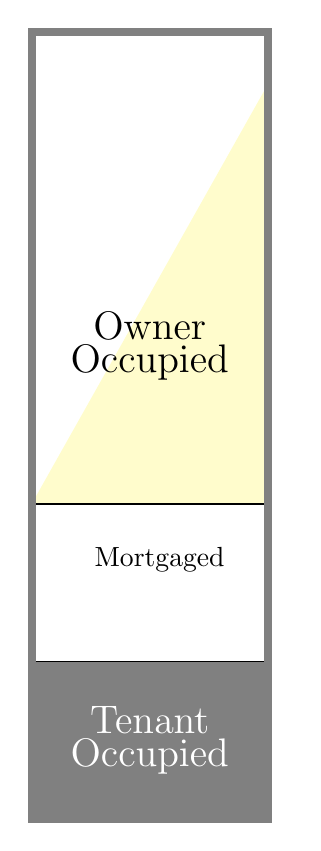
\begin{tikzpicture}{scale=.5}
%   \coordinate (planning) at (-5,1);%PREFACE
% \coordinate (economics) at (5,.75);%
%  \coordinate (geography) at (-.5,-2); %history
% \coordinate (finance) at (0,5); %  
\draw [fill=gray,] (0,0) rectangle (3,2); %TENANT


\draw [fill=yellow!20] (0,4)--(3,4)--(3,9.33); --cycle;% MORTGAGE %Calculation. 80\%owner, so  8 above the tenant line. 2/3*8=5.333. 5.333+2=



\draw[line width= 1mm, black!50] (0,0) rectangle (3,10);

\node at (1.5,6)
    [text width=2.4cm, align=center]
    {\baselineskip=20pt\Large Owner Occupied};
\node at (2,3.3)
    [text width=2.4cm]
    {\baselineskip=20pt Mortgaged};
\node at (1.5,1)
    [text width=2.4cm, align=center, white]
    {\baselineskip=20pt\Large Tenant Occupied};
\end{tikzpicture}
\end{center}

Figure: Housing Tenure 

The mortgage demonstrates the two aspects of financial instruments. It is both a financial instrument that enables  purchase and a financial asset that can be bought and sold. When we consider urban housing, it is the right to future income generated by capital, labour and the city itself through the agglomeration effects that drive productivity. It is an instrument that indirectly captures a share of the urban rents. As productivity rises, wages rise, rents rise, property prices rise and mortgages rise. 

For urban theory and policy formation it is important to distinguish between financial instruments that enable production of real assets, and instruments like  mortgages that primarily facilitate the transfer of real assets or rights to real estate  income. Housing developers borrow to purchase land for development and builders borrow to finance construction. While important, the financial instruments involved are not driving the financialization of housing.  The size of the loans involved is affected by the amount of land purchased and the potential rents earned by that land, but the degree of non-occupant ownership is not affected. *** CLARIFY
  
\begin{center}
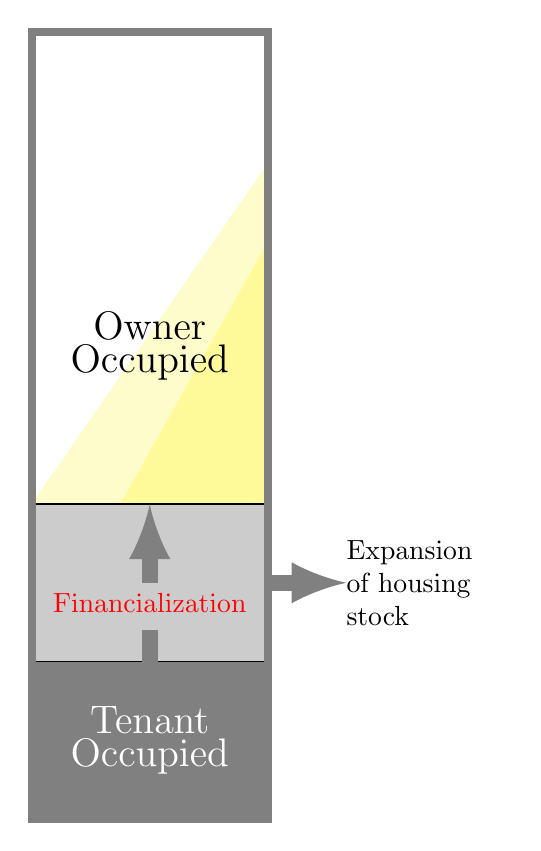
\begin{tikzpicture}{scale=.5}
\draw [fill=yellow!20] (0,4)--(3,4)--(3,8.33); --cycle;% MORTGAGE %Calculation. 80\%owner, so  8 above the tenant line. 2/3*8=5.333. 5.333+2=

\draw [fill=yellow!40] (0,2)--(3,2)--(3,7.33); --cycle;% MORTGAGE %Calculation. 80\%owner, so  8 above the tenant line. 2/3*8=5.333. 5.333+2=
 \draw [fill=gray!40,opacity=1] (0,0) rectangle (3,4); %fiancialization   
\draw [fill=gray] (0,0) rectangle (3,2); %TENANT

\draw[line width= 1mm, black!50] (0,0) rectangle (3,10);

\node at (1.5,6)
    [text width=2.4cm, align=center]
    {\baselineskip=20pt\Large Owner Occupied};
%\node at (2,3.3)
    [text width=2.4cm]
    {\baselineskip=20pt Mortgaged};
    


\node at (1.5,1)
    [text width=2.4cm, align=center, white]
    {\baselineskip=20pt\Large Tenant Occupied};


%\draw [gray,line width=2mm](1.5,2)--(1.5,2.4) node[above, red]{Financialization}; 
\draw [gray,line width=2mm](1.5,2)--(1.5,2.4) node[above, red]{Financialization}; 
\draw [gray,-latex, line width=2mm](1.5,3)--(1.5,4);
\draw [gray,line width=2mm,-latex](3,3)--(4,3); \node at (5,3)[text width=2cm]{Expansion of housing stock}; 

\end{tikzpicture}
\end{center}

Figure: Financialization vs expansion of the housing stock 

\subsection{Investment trusts}

An example of a financial instrument designed specifically to support rent extraction and which  increases the degree of financialization of the housing supply is the  Real Estate Investment Trust (REIT).  A REIT is a company that owns, operates, or finances income-generating real estate and distribute the income to shareholders. There are other large owners of residential real estate such as life insurance companies and pension plans that behave similarly, but REITs are a relatively new financial instrument which is  expanding rapidly and attracting political attention for their effect on housing markets.  % REITs that develop new properties generally don't sell the properties they construct.

REITs have become increasingly popular in recent years.  An S\&P-Dow Jones research bulletin reported that over the  25 years to 2017, REITs outperformed stocks, bonds, and commodities \cite{Dow-Jones-research-bulletin}. Because they have outperformed competing investments they have attracted  capital from other uses.

Developed in the USA  in 1960 (as an amendment to the Cigar Excise Tax Extension) and in Canada in 1993 \cite{REITsDevelopedDates}, REITs are similar to mutual funds in making it possible for an individual, often small investors to earn dividends from real estate investments without having to buy, manage, or finance any properties themselves. There are questions about preferential tax treatment, and whether some REITs are really inappropriately sheltered real-estate corporations.  For the purpose of this thesis, they are simply one of the mechanisms for the financialization of housing.

They are not simply a neutral tool for saving however. According to a paper \cite{wangAnalyzeImpactREITs2021} on REITS in the Irish housing market, ``REIT successfully reconnected the international financial market and the Irish real estate market.'' In other words, in Ireland, REITS have made it easier for international capital to buy Irish land. The entry of outside and footloose capital has had an effect on the resident population:  ``the large-scale acquisition of Irish real estate by REITs and other real estate buyers has also caused some new problems. First, the active management of assets by REITs and other investors has led to a rapid increase in rents''.\footnote{%In IMF working paper \cite{IMF-WP-2015}/15/243 2015, Capital Account Liberalization and Inequality, 
Davide Furceri and Prakash Loungani found that for 149 countries from 1970 to 2010, ``after countries take steps to open their capital account, an increase in inequality in incomes within countries follows'' \cite{furceriCapitalAccountLiberalization2015}. The observation is consistent with our argument  that domestic rent-seeking in housing markets will increase inequality.}   

There is evidence that REITs affect real estate markets in other ways. A \href{https://www.ineteconomics.org/research/research-papers/the-role-of-public-reits-in-financialization-and-industry-restructuring}{report} from the Institute for New Economic Thinking, for example, argues that ``The evidence in this report shows that they are actually financial actors that aggressively buy up property assets and manage them to extract wealth at taxpayers’ expense. ''\footnote{The Role of Public REITs in Financialization and Industry Restructuring. Rosemary Batt and Eileen Appelbaum, with Tamar Katz* Working Paper No. 189 July 9th, 2022} ``\dots they have expanded the pool of capital available for transactions that monetize real property and turn it into tradable assets – financial widgets with little or no connection to the real purpose of the productive enterprises that occupy the properties they own.''

\subsection{Financialization and productivity}

When  a productive asset is acquired as a financial asset it remains productive. %African land or land in Northern Ontario 
Land acquired by holding companies may even be made more productive. 
% the goal of such investments, however, is generally to achieve a capital gain over time. Financial analysis is essentially about rates of return on financial capital invested. The opportunity for capital gains  attracts financial capital to the housing market.%Financial managers have no interest is n in assets that are not expected to increase in value. 


% The financialization of urban housing benefits a globally distributed rentier class of urban landholders. We will make this more explicit below the incentive structure deriving the further financialization of the housing market.

*IT WOULD BE HELPFUL TO CONNECT FINANCIALZATION TO KEY THREAD FROM PAST CHAPTERS AT SOME POINT EVEN IF BRIEFLY